%# -*- coding: utf-8-unix -*-
%%==================================================
%% chapter03.tex for SJRU Master Rhesis
%% implementation2
%%==================================================
%\bibliographystyle{sjtu2}%[此处用于每章都生产参考文献]

\theoremstyle{definition}
\newtheorem{definition}{定义}[section]

\chapter{相似轨迹查询方法实现}
\label{chap:implementation}

\section{相似轨迹查询问题描述}
\label{sec:question describe}
相似轨迹查询传统意义上是根据一条已有历史轨迹,在轨迹数据库中查询出与这一条轨迹在地理位置上形状相似的一条或多条轨迹。在本文中,我们将输入轨迹进一步简化为一组轨迹查询点集$Q$。$Q$在地理位置上保留轨迹原有的形状,通过对点集$Q$进行\emph{k最佳连接}查询,从轨迹数据库$D$中得出k条最相似的轨迹集合$T'$作为输出。由于系统设计与用户的交互,性能指标方面查询结果应满足高效、实时且具有良好的准确性。

\section{k最佳连接定义}
\label{sec:k-bct}
一个轨迹数据库中存储了大量的原始车载GPS轨迹或是已经预处理过的车载GPS轨迹。这里的轨迹由一系列的地理位置点组成$\{p_{1},p_{2},p_{3},\cdots, p_{m}\}$,其中$p_{i}$ $1\leq i \leq m$代表一个由经度和维度构成的地理位置点而$m$代表轨迹中点的数目。本文所定义的k最佳连接查询(k Best-Connected Rrajectory Query)的输入由一组查询点$Q$组成。$q_{j}$ $1 \leq j \leq n$和$p_{i}$定义相同,其中n是查询点的数目。这里用户可以选择选择是否在查询中指定轨迹连接依照查询点的先后顺序,即是否选择查询有序性。若选择查询有序性,则查询点集$Q$为认为是从$q_{1}$到$q_{m}$有序点集。
\begin{displaymath}
	Q = \{q_{1},q_{2},q_{3},\cdots, q_{n}\}
\end{displaymath}

在搜索最好连接轨迹这一上下文中,相似度方程的定义需要和传统方法有所不同,在这里我们将相似度方程定义为一条轨迹连接查询点的好坏程度。因此,本文首要考虑一条轨迹到每一个查询点的距离,我们简要定义距离一个查询点$q_{i}$到一条轨迹$R=\{p_{1},p_{2},p_{3},\cdots, p_{m}\}$的距离为$D_{q}$,即

\begin{equation}
	\label{eq3-1}
	D_{q}(q_{i}, R) = \min_{p_{j} \in R} \{D_{e}(q_{i}, p_{j})\} 
\end{equation}

式\ref{eq3-1}中,$D_{e}(q_{i}, p_{j})$是指查询点$q_{i}$和轨迹点$p_{j}$之间的欧氏距离,因此通常意义上相似度距离$D_{q}$代表从查询点$q_{i}$到轨迹上任一一点距离的最短距离。当我们找到轨迹上一点$p_{j}$是离查询点$q_{i}$的最短距离点时,我们将$<q_{i},p_{j}>$作为最短匹配点对。在无序查询点击中,我们定义查询点集$Q$和轨迹$R$之间的相似度为$Sim(Q,R)$。

\theoremstyle{definition}
\begin{definition}
	轨迹$R={p_{1}, p_{2}, \cdots, p_{n}}$而查询点为$q$,$<q, p_{i}>$表示一组匹配点对。对于$\forall p_{i} \neq p_{j}$, $d_{e}(p_{i}, q)\leq d_{e}(p_{j}, q)$,那么$<p_{i}, q>$是轨迹$R$到查询点$q$的最短匹配点对。
\end{definition}

\begin{equation}
	\label{eq3-2}
	Sim(Q,R) = \sum_{i=1}^{n} \emph{e}^{-D_{q}(q_{i}, R)}
\end{equation}

式\ref{eq3-2}将每个查询点对$Sim(Q,R)$的贡献值通过自然对数去反得以体现,即根据自然函数的单调性,查询点离轨迹越近,则$-D_{q}(q_{i}, R)$越大,以自然对数为底取幂的值也越大,最后使得$Sim(Q,R)$的值也越大。从用户人为角度和地理语义角度上看,一条轨迹与所有的查询点被定义为相似当且仅当这条轨迹和所有的查询点都十分接近。

图\ref{similarity}通过距离说明查询点和轨迹之间的匹配关系。如图\ref{similarity}(a)所示,查询点$q_{1}$、$q_{2}$和$q_{3}$分别与轨迹R上的轨迹点$p_{6}$、$p_{4}$和$p_{7}$最近匹配,根据式\ref{eq3-2}可以得出,$Sim(Q,R) = \emph{e}^{-D_{q}(q_{1}, p_{6})} + \emph{e}^{-D_{q}(q_{2}, p_{4})} + \emph{e}^{-D_{q}(q_{3}, p_{7})} = \emph{e}^{-1.5}+ \emph{e}^{-0.1} + \emph{e}^{-0.1}$。

另一方面,选择查询点和轨迹之前进行有序查询时,顺序性是需要在查询过程中予以考虑。对于查询点$q_{i}$而言,最近匹配点或许并不在是距离上最近的轨迹点$p_{j}$。因此,相似度方程在此步骤中应该适当调整。我们再借用图\ref{similarity}\cite{chen2010searching}予以说明。假设以下用户场景:用户希望查询出一条以$q_{1} \rightarrow q_{2} \rightarrow q_{3}$为顺序的相似轨迹,显然图\ref{similarity}(a)中的顺序并不再符合用户需求。实际的有序查询结果顺序如图\ref{similarity}(b)是$p_{3} \rightarrow q_{4} \rightarrow q_{7}$。在考虑有序性的相似查询规程中,我们的目标是在保持查询有序性的同时追求每一对匹配点对相似度的最大贡献值,即从图\ref{similarity}(b)可以看出$<q_{1},p_{3}>, <q_{2},p_{4}>, <q_{3},p_{7}>$这样的三对匹配点是所有有序匹配对中使得相似度最大的情况。

\begin{figure}[!htp]
  \centering
  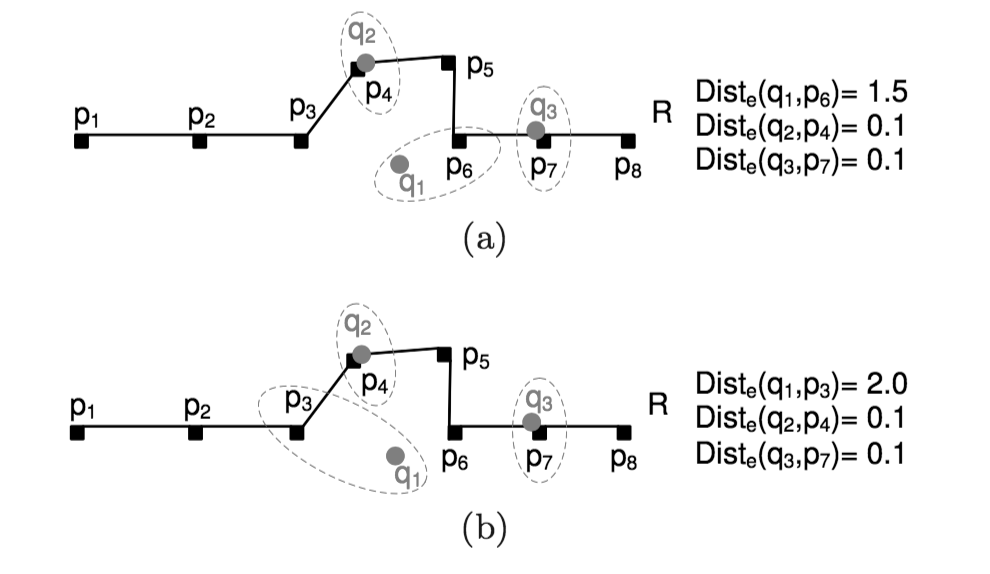
\includegraphics[width=0.7\textwidth]{chapter03/similarity.png}
  \bicaption[similarity]{查询点与轨迹点之间的匹配}{查询点与轨迹点之间的匹配\cite{chen2010searching}}{Fig}{Match between query points and trajectory point}
\end{figure}

有序查询的相似性计算和无序查询也有区别。给定一组有序的查询点$Q_{o} = \{q_{o1},q_{o2},q_{o3},\cdots, q_{on}\}$和一条已有轨迹$R$,我们通过递归思想为有序查询重新定义相似度方程为$Sim_{o}(Q,R)$,式\ref{eq3-3}。其中$Head(x)$函数代表$x$中的第一个点,例如$Head(Q)$是查询点$q_{1}$;同时$Rest(x)$表示$x$去掉x第一个点之后剩余的部分,例如$Rest(Q)$代表\{$q_{2},q_{3},\cdots, q_{n}$\}。在式\ref{eq3-3}中,通过递归的想法,本文将对$Sim_{o}(Q,R)$的求最大值问题分为对两个子问题的求解,即分别计算$Sim_{o}(Rest(Q),R)$和$Sim_{o}(Q,Rest(R))$的最大值问题。当$Head(Q)$和$Head(R)$的两个轨迹点匹配的时候,我们可以将$e^{-D_{e}(Head(Q), Head(R))}$提前计算并加入当后面计算的$Sim_{o}(Rest(Q),R)$之中。在这种情况下,$Head(R)$需要为下一轮的比较计算继续保留,因为对于$Rest(Q)$中的查询点来说,$Head(R)$依旧有可能成为最佳匹配点。而当当$Head(Q)$和$Head(R)$不匹配的时候时我们则跳过$Head(R)$计算$Sim_{o}(Q,Rest(R))$。这种求解思路类似于动态规划的思路,这也为我们再后面优化过程中通过动态规划的来解决这一问题提供了参考。式\ref{eq3-3}结合了动态时间规整(DTW)利用重复点和最长公共子序列(LCSS)省略不匹配点的优点来计算相似度方程。

\begin{equation} 
\label{eq3-3} 
Sim_{o}(Q,R)= max \left\{  
	\begin{array}{lr}  
    e^{-D_{e}(Head(Q), Head(R))} + Sim_{o}(Rest(Q),R) & \\
    Sim_{o}(Q,Rest(R)) &  
    \end{array}  
\right.  
\end{equation}  

根据相似度方程,本文可以对k最佳连接查询有以下定义3.1.2.:

\theoremstyle{definition}
\begin{definition}
	给定一组轨迹集合 $T = {R_{1}, R_{2}, R_{3} \cdots, R_{n}}$、一组查询点$Q = {q_{1},q_{2},q_{3},\cdots, q_{n}}$和对应的相似度方程$Sim$,k最佳连接查询则可以从轨迹集合$T$中找到k条轨迹$T'$,满足式\ref{eq3-4}。其中$Sim$根据用户定义选择是否考虑有序性。:
	\begin{equation}
		\label{eq3-4}
		Sim(Q,R_{i})_{R_{i} \in T'} \geq Sim(Q,R_{j})_{R_{j} \in T-T'}
	\end{equation}
\end{definition}

在进行有序查询的过程中,之前的算法是基于递归进行实现的:通过去不断匹配轨迹和查询点来进行子递归,从而计算出轨迹和有序查询点集之间的相似度大小。但基于递归相似度计算会占用大量的时间。因此在本上,我们通过动态规划的思路来计算某一条轨迹$R$和查询点集$Q$的相似度,借此来优化算法在有序查询中的处理性能。

\begin{algorithm}
%\begin{algorithm}[htp] % 强制定位
\caption{有序相似度算法dp\_Similarity(Q,R)}
\label{algo:dp-sim}
\begin{algorithmic}[1] %每行显示行号
\Require 查询点集$Q={q_1,q_2,q_3,\cdots,q_m}$,轨迹$R={p_1,p_2,p_3,\cdots,p_n}$
\Ensure 查询点集$Q$和轨迹$R$之间的有序相似度$Sim_{order}(Q,R)$
\State Initialise 2-dimensional array $M[m+1][n+1]$;
\State $M[i][0] \gets 0$ $for$ $1\leq i\leq m$;
\State $M[0][j] \gets 0$ $for$ $1\leq j\leq m$;
\For{$1\leq i\leq m$} 
	\For{$1\leq j\leq n$}
		\If{$e^{-D_{e}(Head(Q),Head(R))} + M[i-1][j] > M[i][j-1]$}//$q_i$和$p_j$匹配
		\State $M[i][j] \gets e^{-D_{e}(Head(Q),Head(R))} + M[i-1][j]$; //重复$p_j$
		\Else 
		\State $M[i][j] \gets M[i][j-1]$; //略过$p_j$
		\EndIf
	\EndFor
	\State \textbf{return} M[m][n]$\setminus n$;
\EndFor
\end{algorithmic}
\end{algorithm}

假设$M[i][j]$是我们需要解决查询问题的子问题的有序相似度,即$Sim_{order}(\{q_1,q_2,q_3,\cdots,q_i\}$, $\{p_1,p_2,p_3,\cdots,p_j\})$。对于动态规划思路而言,当我们获取到$M[i-1][j]$和$M[i][j-1]$的值时,我们可以通过比较$e^{-D_{e}(Head(Q),Head(R))} + M[i-1][j]$和$M[i][j-1]$的值来决定$M[i][j]$的最大值。如果值$e^{-D_{e}(Head(Q),Head(R))} + M[i-1][j]$较大,我们可以得出目前的一对匹配点对为$<p_i, p_j>$,并令$M[i][j] = e^{-D_{e}(Head(Q),Head(R))} + M[i-1][j]$,反之,我们略过对$p_j$的目前和之后匹配,并令$M[i][j]=M[i][j-1]$。由于历史轨迹点的数目各不相同,对于重复使用的点,我们需要将相似度计算结果正则化以符合实际。

这一动态规划的思路自底向上的解决了$M[i][j]$的求值问题,其中$m$为查询点集的基数大小而$n$为轨迹点数目。在算法最后通过范围二维数组中的值来表示查询点集$Q$和轨迹$R$之前有序相似度。算法的复杂性为$O(mn)$,在具体应用中由于$m$的值相对于$n$来说普遍较小,所以我们可以将算法复杂性近似看成是线性的。

\section{相似轨迹查询处理过程}
\label{sec:query processing}

\subsection{算法变量符号定义及解释}
\label{subsec:algorithm-definition-explanation}
表\ref{tab-notations}提供了本文本章节之后所涉及的基本符号及其注释。

\begin{table}[!htpb]
  	\centering
		\begin{tabular}{ |p{1.5cm}||p{5.5cm}|p{1.5cm}||p{5.5cm}| }
		\hline
		符号标记 & 符号注释 & 符号标记 & 符号注释\\
		\hline
		$N$ & 一条轨迹的轨迹点总数目 & $m$ & 一组查询点总数目\\
		\hline
		$D_{e}(q_{i},p_{j})$ & 点$q_{i}$和点$p_{j}$之间的欧氏距离 & $C$ & 轨迹备选集 \\
		\hline
		$D_{e}(q_{i},p_{j})$ & 点$q_{i}$和点$p_{j}$之间的欧氏距离 & $\epsilon$ & 搜索范围阈值\\
		\hline
		$D_{q}(q_{i},R)$ & 点$q_{i}$和轨迹$R$之间的最短距离 & $\rho$ & 轨迹点密度 \\
		\hline
		$r$ & $\lambda$-NeareatNeighbor搜索半径 & $\xi$ & 查询点$q_{i}$对相似度上界贡献\\
		\hline
		$\mu,\upsilon$ & 优化搜索权值 & $UB_{ns}$ & 未在备选集中轨迹的相似度上界\\
		\hline
		$LB$ & 备选集中轨迹的相似度下界 & & \\
		\hline
		\end{tabular}
	\bicaption[tab-notations]{公式符号列表及其对应注释}{本文符号列表及其对应注释}{Table}{A list of notations and explanations}
\end{table}


\subsection{相似轨迹查询问题概述}
\label{sec:problem Forumation}
轨迹数据为一组有序点集,轨迹$R$可以被表示为$R={p_{1}, p_{2}, \cdots, p_{n}}$,其中$p_{i}$是轨迹$R$的在时间顺序上的第$i$个轨迹点。对于本文应用而言,查询点集$Q$被定义为一组点集$Q={q_{1}, q_{2}, \cdots, q_{m}}$,且根据具体情况定义是否有序。在根据上文设计的相似性距离和k最佳连接定义后,我们将我们相似轨迹查询任务等价转化为k最佳连接查询,并产生下面的定义:

%\theoremstyle{definition}
\begin{definition}
	给定已有的轨迹数据集$D$,和一条待查询轨迹$R_{q}$。我们通过轨迹简化算法\cite{visvalingam1990douglas,chen2009trajectory}将待查询轨迹$R_{q}$转换成一组查询点集$Q$。通过k最佳连接查询方法,从轨迹数据集$D$中获取k条轨迹,集合为$D' = {R_{1}, R_{2}, \cdots, R_{k}}$,满足式\ref{eq3-5}。其中$Sim$根据用户定义选择是否考虑有序性。:
	\begin{equation}
		\label{eq3-5}
		Sim(Q,R_{i})_{R_{i} \in D'} \geq Sim(Q,R_{j})_{R_{j} \in D-D'}
	\end{equation}
	我们称$D'$轨迹数据集合为对于轨迹$R_{q}$的k条最相似轨迹查询结果。
\end{definition}

\subsection{相似轨迹查询算法实现}
\label{subsec:algorithm implementation}

\begin{figure}[!htp]
  \centering
  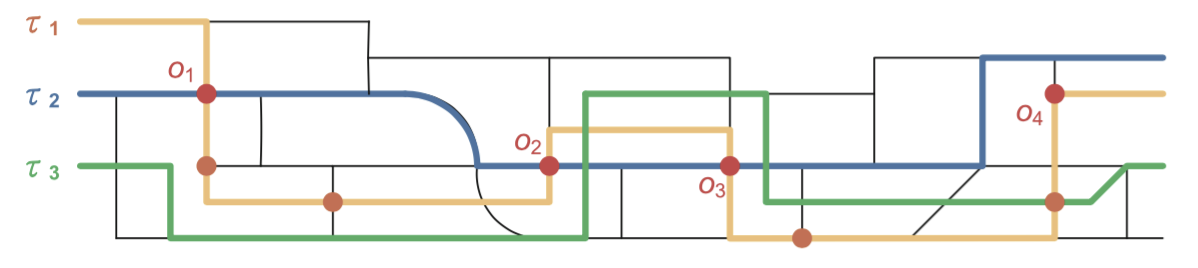
\includegraphics[width=0.8\textwidth]{chapter03/similar-search.png}
  \bicaption[fig:similar-search]{基于位置点的相似轨迹查询}{基于位置点的相似轨迹查询\cite{shang2014personalized}}{Fig}{Search similar trajectory by location points}
\end{figure}

如图\ref{fig:similar-search}\cite{shang2014personalized}所示,本文所实现的相似轨迹查询算法主要为针对地理位置点集的轨迹搜索算法\cite{qi2015efficient}。将轨迹数据按特定需求分类索引在R树数据结构上后,该相似轨迹查询算法在轨迹点k最近邻查询算法\cite{roussopoulos1995nearest}基础上,实现了增长型k最近邻查询算法\cite{chen2010searching},结合备选和筛选(candidate-refinement)的剪枝思路\cite{tang2011retrieving},通过轨迹相似度上界与下界对搜索空间进行优化处理,以满足空间搜索算法的高效性和准确性。

在这里,轨迹相似度上界与下界所满足的搜索剪枝关系用定理\ref{thm:similarity-bound}描述

\begin{thm}[相似度上下界]
	\label{thm:similarity-bound}
	假设对于相似轨迹插叙的k最佳连接算法没有有序性限制,我们可以在对查询点集进行一轮k最近邻查询(k=$\lambda$)之后的轨迹备选集C中,选取一个包含k条轨迹的一个轨迹子集$C'$。当$\min_{R_{x}\in C'}{LB(R_{x})}\geq UB_{us}$这一条件满足时,我们可以从轨迹备选集$C$中获得k条最佳连接轨迹,即k条与查询点集最相似的轨迹。
	\begin{proof}
	首先对于轨迹子集$C'$中的某一条轨迹$R_{a}$($R_{a} \in C'$)而言,轨迹$R_{a}$满足$Sim(Q,R_{a}) \geq LB(R_{a})$。与此同事,对于轨迹备选集$C$之外的轨迹$R_{b}$($R_{b} \notin C$),轨迹$R_{b}$满足$UB_{ns} \geq Sim(Q,R_{b})$。当上述定理成立时,即$\min_{R_{a}\in C'}{LB(R_{a})}\geq UB_{ns}$,我们可以推断出$\forall R_{a}\forall R_{b} \big( R_{a} \in C' \wedge R_{b} \notin C \big)$,$Sim(Q,R_{a}) \geq Sim(Q,R_{b})$成立。这也证明了对于查询点集$Q$得到的k最佳连接的结果轨迹在这个时候应该全部在轨迹备选集$C$中。
	\end{proof}
\end{thm}

%\begin{algorithm}
%\caption{相似轨迹查询算法}
%\label{algo:iknn}
%\begin{algorithmic}[1] %每行显示行号
%\Require 相似轨迹查询数目$k$, 查询点集$Q$ % 输入
%\Ensure k条最相似轨迹$k$-$Trajs$ % 输出
%\State Candidate Set $C$; //初始化轨迹备选集$C$
%\State Initialise $UB_{ns}$ $LB[]$, $k$-$LB[]$ ; //初始化轨迹相似度上界和相似度下界
%\State $\lambda \gets k$ //将k值初始赋值给$\lambda$
%\While {true}
%	\For{each $q_{i} \in Q$ that $1\leq i\leq m$}
%		\State $C_{i} \gets$ trajectories that contains the points in $\lambda$-$NN(q_{i})$;
%	\EndFor
%	\State $C \gets\bigcup_{i=1}^{m}C_{i}$; //合并轨迹备选子集以生成轨迹备选集C
%	\If {$|C| \geq k$}
%		\State compute $LB[]$ for all trajectories in $C$; //计算轨迹备选集C中的所有轨迹相似度下界
%		\State compute $UB_{ns}$; //计算相似度上界
%		\State $k$-$LB[]\gets$ $LB[]$.heapKtop(); //选取相似度下界k个最大值和其对应的轨迹
%		\If {$k$-$LB[].min\geq UB_{ns}$}
%			\State $k$-$Trajs\gets refine(C)$ //轨迹筛选方法
%			\State \textbf{return} $k$-$Trajs$ 
%		\EndIf 
%	\EndIf
%	\State $\lambda\gets\lambda+\Delta\lambda$;
%\EndWhile
%\end{algorithmic}
%\end{algorithm}


算法{\cite{chen2010searching}}大致流程如图\ref{fig:iknn-flowchart}。通过函数主体首先定义初始化几个中间变量。$while$循环实现增长型k最邻近的每一轮查询。查询中,对查询点集$Q$中的每一个查询点进行k最近邻方法查询,对查询结果中的每一个轨迹点所在的轨迹都加入轨迹备选集$C$。判断轨迹备选集$C$的基数大小是否满足条件。如果满足条件,计算此时归集备选集中所有轨迹的相似度下界大小并用一个数组$LB[]$进行保存,同时计算未在轨迹备选集中的轨迹的相似度上界大小。运用堆排序或优先队列的思想将数组$LB[]$中选取$k$个最大相似度下界及相对应的轨迹。如果\ref{thm:similarity-bound}满足,即选出来$k$条轨迹中的最小轨迹相似度下界大于等于未在轨迹备选集中的轨迹相似度上界,则说明我们需要查询的$k$条最相似轨迹已经存在于轨迹备选集$C$中,并且其他未扫描到的轨迹可以忽略不予以计算与检查。

%\begin{figure}[!htp]
%  \centering
%  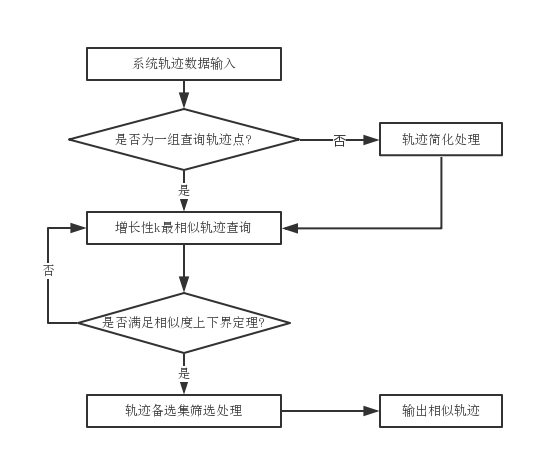
\includegraphics[width=0.8\textwidth]{chapter03/iknn-flowchart.png}
%  \bicaption[fig:iknn-flowchart]{相似轨迹查询算法流程图}{相似轨迹查询算法流程图}{Fig}{Searching algorithm flow chart}
%\end{figure}

\begin{figure}[!htp]
    \centering
    \resizebox{10cm}{!}{
\begin{tikzpicture}[node distance=2cm]

	\node (input) [startstop,font=\bf,fill=green!20] {输入轨迹数据类型判断};
	\node (input_judge) [decision, below of=input,yshift=-0.5cm,aspect=2.5,fill=red!20] {是否为用户指定一组轨迹点集?};
	\node (ts) [process, right of=input_judge,xshift=5cm] {轨迹简化};
	\node (iknn) [process, below of=input_judge,yshift=-0.5cm]{增长型k相似轨迹查询};
	\node (bound_judge) [decision, below of=iknn,yshift=-0.5cm,aspect=2.5,fill=red!20]{是否满足相似度上下界条件?};
	\node (refinement)[process, below of=bound_judge,yshift=-0.5cm]{备选轨迹集筛选};
	\node (output)[startstop, below of=refinement,font=\bf,fill=green!20]{k条最相似轨迹输入};
	

	\draw [arrow] (input) -- (input_judge);
	\draw [arrow] (input_judge) -- node[anchor=south]{否}(ts);
	\draw [arrow] (input_judge) -- node[anchor=west]{是}(iknn);
	\draw [arrow] (ts) |- (iknn);
	\draw [arrow] (iknn) -- (bound_judge);
	\draw [arrow] (bound_judge.west) |- node[anchor=south]{否}(iknn.west);
	\draw [arrow] (bound_judge.south) -- node[anchor=west]{是}(refinement.north);
	\draw [arrow] (refinement) -- (output);
\end{tikzpicture}

}
    \bicaption[fig:iknn-flowchart]{相似轨迹查询算法流程图}{相似轨迹查询算法流程图}{Fig}{Searching algorithm flow chart}
\end{figure}


%%%%%%%%%%


\section{分布式相似轨迹查询算法实现}
\label{sec:distributed algo}
在之前的工作描述中,我们对于相似轨迹查询的实现总会提及查询点集的数目相对较少这一前提。对于单机处理而言,如果将一整条轨迹的轨迹数据点作为输入或者查询点集过多,由于增长型k最近邻查询会对每一个查询点都进行$\lambda$-NN的搜索处理,因此整个相似轨迹的查询过程会显得相对缓慢。但有些时候,将一条轨迹作为相似轨迹查询的输入的确更简单且更人性化\cite{shang2014personalized}。在硬件设置对算法性能的约束下,借助基于地理位置点的轨迹简化方法,我们可以对前一章所涉及的相似轨迹查询方法通过加入\emph{Spark}分布式集群处理的手段,做到以一条轨迹(或数量更多的查询点)为输入的相似轨迹查询操作。具体实现思路在于,通过基于地理位置点的轨迹简化方法将一条轨迹简化为一组数量相对于单机查询要多的查询点集;然后将查询点通过分布式集群操作分配给各个子节点来进行相对于各集群节点的相似轨迹查询操作,各个子节点通过访问HDFS获取轨迹数据和轨迹R树索引;最后将结果以轨迹为关键字,以相似度为权值进行求和,选择相似度和最高的k条轨迹作为查询结果。


\subsection{Spark分布式相似轨迹查询}
\label{subsec:distributed similar}
\emph{Spark}集群环境使得我们可以将代码分发给各个工作节点使他们处理对数据集相同的操作,这为分布式搜索相似轨迹提供了实现的基础。单机实现相似轨迹搜索为保证运行性能,给定的输入集查询点需要保证数量在某一程度上相对较小。但对于分布式处理而言,这一约束可以通过集群集计算处理予以取消。给定一条原始轨迹$Traj$,我们可以先通过基于地理位置点的轨迹简化在保留轨迹形状和轨迹中的重要位置点的同时,一定程度上减少轨迹数目。事实上,如果集群设备性能较好,我们可以略去集群计算相似轨迹前对轨迹简化这一步骤。由于本文实验设备限制,通过在集群处理前的轨迹简化能在保证结果正确性的过程中,稳定处理性能。因此,我们将轨迹简化作为集群计算前的预处理过程。

\begin{figure}[!htp]
  \centering
  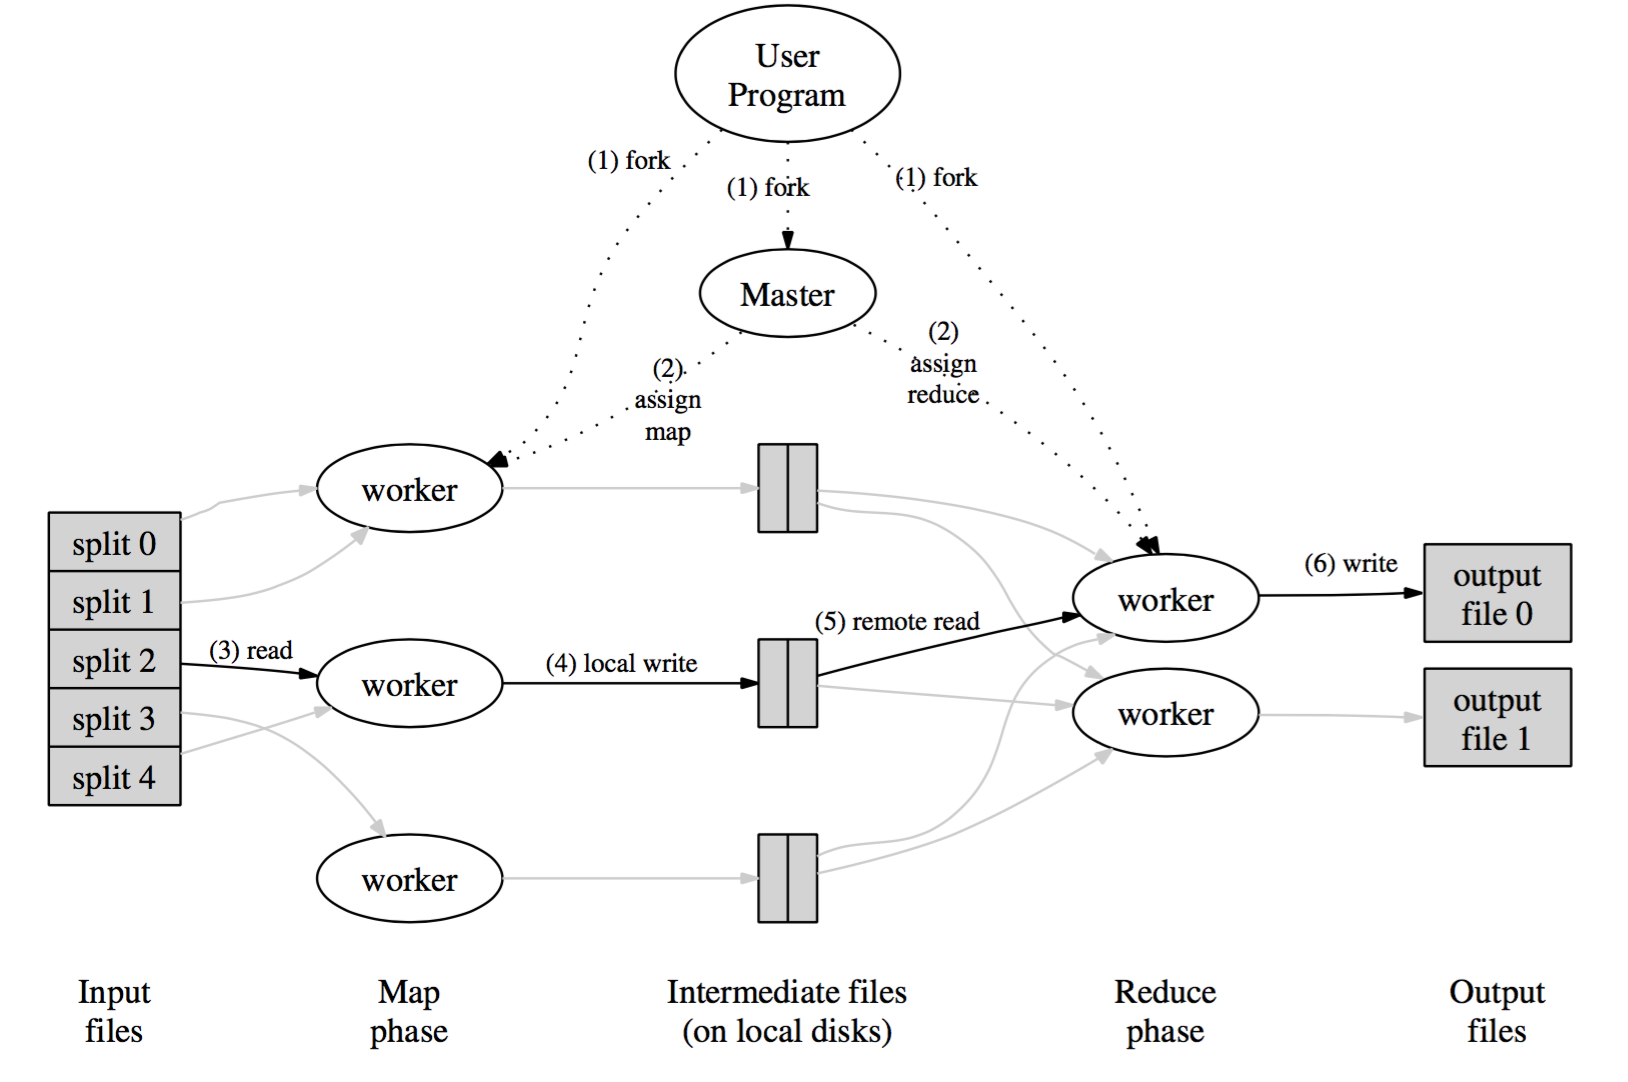
\includegraphics[width=0.8\textwidth]{chapter04/distributed.png}
  \bicaption[fig:distributed]{Spark分布式相似轨迹查询流程}{Spark分布式相似轨迹查询流程\cite{dean2008mapreduce}}{Fig}{The flow of Spark distributed search similar trajectories}
\end{figure}

图\ref{fig:distributed}\cite{dean2008mapreduce}为\emph{MapReduce}的大致处理框架,我们根据这一框架设计出分布式查询相似轨迹的大致算法。在算法中,假设我们已经完成对原始轨迹的简化得到已处理好的简化轨迹$Traj'$\cite{chen2009trajectory}。首先我们通过\emph{Spark}内的\emph{partition}函数将输入数据分割,并分发给每一个工作节点(\emph{Worker Node})。对于每一个工作节点而言,他们都有了输入数据的一部分轨迹点。对于每一个工作节点而言,他们都可以将自己所拥有的部分轨迹点作为相似轨迹查询的查询点集,由于工作节点通过设置可以直接访问\emph{HDFS}上已存储的轨迹数据,我们通过主节点(\emph{Master Node})将增长型k最近邻查询代码分发给每一个工作节点并予以上运行。每个工作节点将针对各自输入查询点集所得出的k条最相似轨迹及其对应的相似度大小作为输出。通过对轨迹作为关键字合并中间查询结果,对相似度求和按相似度大小降序排列轨迹,再从中选取k条轨迹作为最终的结果。

实现细节如算法\ref{algo:distributed sim}所示。其中在运行过程中初始化\emph{Spark}运行所需的上下文变量并设置主节点信息。在\emph{map}阶段对查询点集进行查询搜索,在\emph{reduce}阶段进行关键字合并。

\begin{algorithm}
% \begin{algorithm}[H] % 强制定位
\caption{分布式相似轨迹查询算法}
\label{algo:distributed sim}
\begin{algorithmic}[1] %每行显示行号
\Require 相似轨迹查询数目$k$,一条原始轨迹数据$Traj$% 输入
\Ensure $k$条最相似轨迹$k$-$Trajs$ % 输出
\State $Traj' \gets TS(Traj)$; $\qquad$//简化轨迹
\State Initialise \emph{Spark} Context $sc$ and set Master information;
\State $RDD \gets sc.parallelize(Traj', partitionNumber)$;
\State $k$-$Trajs$ $\gets RDD.map(iknn) $ $\qquad$//工作节点分布式进行查询处理
\State $\qquad\quad.flatMap(lambda\quad x$:$x)$ $\qquad$//查询结果平铺成为一维列表或数组
\State $\qquad\quad.reduceByKey(lambda\quad x,y$:$x+y)$$\qquad$//以轨迹为关键字做相似度求和
\State $\quad\qquad.sortBy(lambda\quad x$:$x[1], descending)$$\qquad$//降序排列
\State $\quad\qquad.collect()$;
\State \textbf{return} $k$-$Trajs$; 
\end{algorithmic}
\end{algorithm}

\subsection{多请求分布式相似轨迹查询}
\label{subsec:distributed multiple}
从工业应用角度,多用户同时进行相似轨迹处理时,可以针对对多请求的分布式相似轨迹查询处理。将请求数据集根据\emph{Spark}环境默认的分割方法或自定义的分割方法,将多请求分割成多个子集,然后分配个集群中的子节点,让他们各自处理处理一部分请求。在实际生活中,作为一个交付使用的应用,在某个时段可能有多个用户请求发送给服务器端,在配置有集群环境的情况下,可以实现对请求的分布式处理,具体思路类似于上文分布式相似轨迹查询,不予以赘述。


%%%%%%%%%%


%\section{算法优化}
%\label{sec:optimization}

%\subsection{$\lambda$动态增长优化}
%\label{subsec:lambda}

%在增长型k最近邻查询算法中,对于每一次的k最近邻查询$\lambda$-NN($q_{i}$)而言,搜索范围$\lambda$都是动态增加$\Delta\lambda$,即每一轮循环中,对于查询点集中的每一个查询点$q_{i}$,搜索范围在数目上是相等的。但值得提出的时,在针对地理位置点进行相似轨迹查询这一上下文中,查询点对于结果的重要性并不是完全一致的。主观而言,有些位置点相对于其他位置点来说具有更重要或更优先的查询级别;从算法角度讨论,每个查询点$q$的结果$\lambda$-NN($q$)对于构建轨迹备选集$C$、决定轨迹相似度上下界均有着不同的影响程度。举例来说,对于两个查询点$q_{i}$和$q_{j}$,在$\lambda$相同的情况下,如果$D_{e}(q_{i}, p_{i}^{\lambda}) > D_{e}(q_{j}, p_{j}^{\lambda})$,则对于查询点$q_{i}$所查找的范围更大,即$e^{-D_{e}(q_{i}, p_{i}^{\lambda})} < e^{D_{e}(q_{j}, p_{j}^{\lambda})}$。根据,$UB_{ns} = \sum_{i=1}^{m}e^{-D_{e}(q_{i}, p_{i}^{\lambda})}$,我们可以根据结果推出在降低未在备选集中的轨迹相似度上界的过程中,查询点$q_{i}$比查询点$q_{j}$效果更好,更有帮助。在定理3.1.2.中,未在备选集中的轨迹相似度上界越低,则定理条件越容易满足,即增长型k最近邻查询算法可以更快得出结果。我们需要分析$\lambda$对每个查询点搜索的影响来决定如何动态增加搜索范围。首先我们定义每个查询点$q_i$对于$UB_{ns}$的影响为$\xi (q_i)$

%\begin{displaymath}
%	\xi (q_i) = e^{-D_{e}(q_i,p_i^\lambda)}
%\end{displaymath}
%显然,当$\xi (q_i)$的值越小时,则相对应的$UB_{ns}$也将越小。接着我们定义$\rho$为某一范围内轨迹点的密度值,定义$r=D_{e}(q_i,p_i^\lambda)$为对查询点$q_i$进行k最近邻查询时的搜索半径。在k最近邻查询这一范围内,我们可以粗略计算出轨迹点的密度值$\rho$等于

%\begin{displaymath}
%	\rho = \frac{\lambda}{\pi r^{2}}
%\end{displaymath}
%根据轨迹点密度和搜索半径的关系,我们重写$\xi (q_i)$为

%\begin{displaymath}
%	\xi (q_i) = e^{-D_{e}(q_i,p_i^\lambda)} = e^{-r} = e^{-\sqrt{\frac{\lambda}{\pi\rho}}}
%\end{displaymath}
%在这一步,我们的首要目标是明确$\xi (q_i)$影响因子的下降速度与$\lambda$之间的关系,根据$\lambda$的变化所造成的影响赋予查询点$q_1$到$q_m$不同的$\Delta\lambda$变化值,即对于不同的查询点,除了初始第一轮查询之外,之后($\lambda+\Delta\lambda$)的值都是各自生成的。本文将$\xi (q_i)$为关于$\lambda$的微分值$\frac{d\xi}{d\lambda}$的绝对值定义为下降速率$Decay(q_i)$

%\begin{equation}
%\label{eq3-11}
%\frac{d\xi}{d\lambda} = \frac{d}{d\lambda}e^{-\sqrt{\frac{\lambda}{\pi\rho}}} = -\frac{1}{2}(\pi\rho\lambda)^{-\frac{1}{2}}*e^{-\sqrt{\frac{\lambda}{\pi\rho}}}
%\end{equation}
%根据式\ref{eq3-11},我们可以用$\lambda$和搜索半径$r$来计算轨迹点密度$\rho$,因此可以改写下降速率为

%\begin{equation}
%\label{eq3-12}
%Decay(q_i) = |\frac{d\xi}{d\lambda}| = \frac{r}{2\lambda}e^{-r} 
%\end{equation}

%根据式\ref{eq3-12},我们可以得知,对于一个固定的$\lambda$值来说,下降速率$Decay(q_i)$会随着搜索半径$r$的不断增长,先初步上升($r\in(0,1]$)后逐渐下降$r\in(1,\infty)$)。我们可以得知在对于查询结果较为稀疏的查询点(即搜索半径$r$较大)在一开始赋予较大的查询权重值。但随着搜过过程的进行,当搜索半径$r$不断增长达到某一个值得时候,一些相对密集的查询点结果会使得其对应的下降速率变大。这一结论使得我们在搜索和查询过程中重点关注查询点结果较为密集的查询点,这样也能使得我们能更快更有效地在每一轮查询之后降低未在轨迹备选集中轨迹的相似度上界值$UB_{ns}$。但随之产生的问题在于,当搜索半径$r$和$\lambda$都足够大的时候,我们下降$UB_{ns}$会因为$\frac{d\xi}{d\lambda}$趋近于0而变得不再有效。

%满足定理\ref{thm:similarity-bound}需要上下界两个变量对条件的同时满足。因此,在关注未在轨迹备选集中轨迹的相似度上界值$UB_{ns}$对增长型k最近邻查询的影响时,我们可以在加速增长型k最近邻查询算法的时候考虑相似度下界这一因素。当备选集中轨迹的相似度下界$LB$增长越快的时候,定理\ref{thm:similarity-bound}也就越容易成立。提高相似度下界$LB$所要面对的问题在于,一条轨迹的相似度下界有可能是源于多个查询点所产生查询结果,并且想要预测在搜索过程中什么时候$\lambda$-NN($q_i$)的结果中的某一点和轨迹上的某一点恰好是同一个点也是不太容易的。换言之,我们问题主要在于定量描述每一个查询点对于相似度下界增长的影响。借此,我们基于每一轮重新查找到的新轨迹数目来定义一个启发式搜索的取回速率$Ratio(q_i)$
%\begin{equation}
%\label{eq3-13}
%Ratio(q_i) = \frac{Number(q_i)}{\Delta\lambda}
%\end{equation}

%式\ref{eq3-13}中$\Delta\lambda$为当前循环轮次$\lambda$的值与上一轮循环中$\lambda'$值的差值($\lambda > \lambda'$),而$Number(q_i)$表示在当前循环轮次搜索中获取的轨迹数目多少。基本思想在于,轨迹备选集$C$的基数值范会随着搜索过程中新轨迹数目的增长而增长。在这样的归集备选集$C$中,轨迹相似度下界会曾铮的更快,再根据定\ref{thm:similarity-bound},我们也更有可能找到目标寻求的k条最相似轨迹。

%结合考虑上文所提及的下降速率$Decay(q_i)$和取回速率$Ratio(q_i)$,我们可以对每一个查询点指定对应的$\lambda$查询增长值$\Delta\lambda(q_i)$

%\begin{equation}
%\label{eq3-14}
%\Delta\lambda(q_i) = \gamma\big( \alpha\frac{Decay(q_i)}{\sum_{i=1}^{m}Decay(q_i)} + \beta\frac{Ratio(q_i)}{\sum_{i=1}^{m}Ratio(q_i)} \big)
%\end{equation}
%式\ref{eq3-14}中,$\alpha$和$\beta$是本文定义的权值,$\gamma$定义为$\gamma = mk2^{r}$ 其中$r$为算法增长型k最近邻查询的当前循环轮次数。这样,我们摈弃原先对每一个查询点都增长相同的$\lambda$值这一处理思路,选择通过式\ref{eq3-14}的方法应用于每一个查询点上以对每个查询的进行不同的$\lambda$增量处理。这样的预先处理会在挖掘出相对重要的轨迹查询点上花费一定时间,但也加速了整个增长型k最近邻查询算法的搜索过程。这样的预处理时间由于优化整个算法过程,因此是可接受的。注意到我们在每一轮$\lambda$增量的总值是

%\begin{displaymath}
%\sum_{i=1}^{m}\Delta\lambda(q_i)=\gamma\big( \alpha\frac{\sum_{i=1}^{m}Decay(q_i)}{\sum_{i=1}^{m}Decay(q_i)} + \beta\frac{\sum_{i=1}^{m}Ratio(q_i)}{\sum_{i=1}^{m}Ratio(q_i)} \big)=\gamma(\alpha+\beta)
%\end{displaymath}
%为了保证在每一轮增长型k最近邻查询过程中获取的结果轨迹点数据恒定,我们将$\alpha+\beta$设定为1,其中可以设定$\alpha=\beta=0.5$,这样每一轮我们获取的点的数据为$\gamma$

%\subsection{动态规划计算有序轨迹相似度}
%\label{subsec:dp-order-sim}
%在前文中我们提及查询的有序性和用户指定有关。在进行有序查询的过程中,之前的算法是基于递归进行实现的:通过去不断匹配轨迹和查询点来进行子递归,从而计算出轨迹和有序查询点集之间的相似度大小。但基于递归相似度计算会占用大量的时间。因此在本质上,我们通过动态规划的思路来计算某一条轨迹$R$和查询点集$Q$的相似度,借此来优化算法在有序查询中的处理性能。

%假设$M[i][j]$是我们需要解决查询问题的子问题的有序相似度,即$Sim_{order}(\{q_1,q_2,q_3,\cdots,q_i\}$, $\{p_1,p_2,p_3,\cdots,p_j\})$。对于动态规划思路而言,当我们获取到$M[i-1][j]$和$M[i][j-1]$的值时,我们可以通过比较$e^{-D_{e}(Head(Q),Head(R))} + M[i-1][j]$和$M[i][j-1]$的值来决定$M[i][j]$的最大值。如果值$e^{-D_{e}(Head(Q),Head(R))} + M[i-1][j]$较大,我们可以得出目前的一对匹配点对为$<p_i, p_j>$,并令$M[i][j] = e^{-D_{e}(Head(Q),Head(R))} + M[i-1][j]$,反之,我们略过对$p_j$的目前和之后匹配,并令$M[i][j]=M[i][j-1]$。这一动态规划的思路自底向上的解决了$M[i][j]$的求值问题,其中$m$为查询点集的基数大小而$n$为轨迹点数目。在算法最后通过范围二维数组中的值来表示查询点集$Q$和轨迹$R$之前有序相似度。算法的复杂性为$O(mn)$,在具体应用中由于$m$的值相对于$n$来说普遍较小,所以我们可以将算法复杂性近似看成是线性的。

%%%%%%%%%%

\section{本章小结}
\label{sec:implementation conclusion}
本章节在相关工作的基础上,定义了一些轨迹相关的符号变量,并基于这些符号变量和已有的相关工作,从问题的本质出发,设计了基于k最近邻查询的增长型k最近邻算法。通过将k最佳连接查询结果等价视作为k最相似轨迹查询结果,实现相似轨迹查询。在实现过程中,通过对搜索范围的剪枝优化、对搜索参数的动态设定和对查询有序性无序性的特殊处理,结合备选和筛选的处理思路,将相似轨迹搜索过程的处理性能实现在用户可接受范围内。

另一方面,随着如今GPS技术的发展和车载数据的激增,轨迹数据挖掘的数据规模通常较大,因此在处理轨迹数据过程中,单机本地操作或许无法满足轨迹挖掘的特定需求。因此,我们可以通过分布式集群处理的方法来完成大数据轨迹数据挖掘。分布式如今发展较为成熟,为我们提供了许多适应于不同应用的大数据分布式处理框架。根据\emph{MapReduce}的编程模型,我们自定义对输入、中间过程和输出的处理方法,借助分布式框架\emph{Spark}提供的接口方法能够较好的完成本文的相似轨迹查询在分布式上的实现。